\chapter{实验过程}

本次毕业设计“面向智慧交通场景的多目标跟踪算法和评测”中,多目标跟踪技 术作为完成相关功能的核心技术之一,本次研究通过 CARLA 仿真平台中的 Town10 场 景进行实验,优化现有目标跟踪模型并对其进行测试评估。利用跟踪得到的小车轨迹数 据,提高复现性能指标。方法如下。

\section{基础控制}
\subsection{轨迹平滑控制}

假如小车预先设定的路径中,相邻两个路点的距离间隔太大,则小车行驶起来会有很别扭、不自然的感觉,精确操控也较难。轨迹平滑算法可以在原有的路径点间添加几个多余点,令小车轨迹顺畅,如此一来,小车的行驶会流畅不少,如图\ref{fig:p9}。


\begin{figure}[htbp] % 可以是h(here),t(top),b(bottom),p(page of floats)
	\centering
	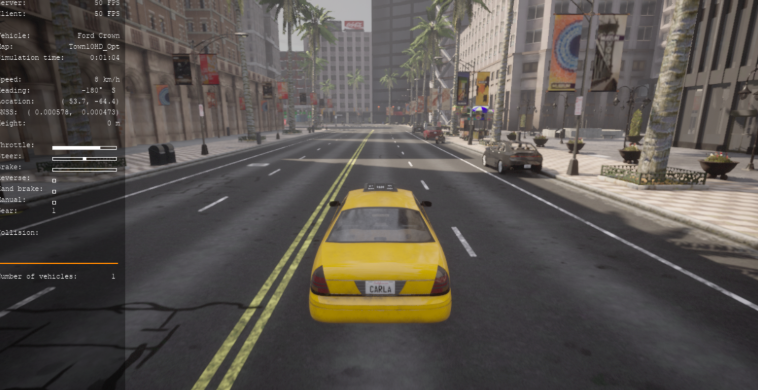
\includegraphics[width=1\textwidth]{p9} % 假设图片文件名为car.pdf或car.png等,位于当前工作目录
	\caption{轨迹平滑控制} % 图片标题
	\label{fig:p9} % 用于引用的标签
\end{figure}






\subsection{实现步骤}

设定最近距离阈值:依据小车的运动学参数以及仿真的环境要求来设定一个最近距离阈值,本课题初期在 Carla 环境中选取的是0.5米。

在需求计算插值点时,首先依次检索原轨迹点,当遇到相邻两点间的距离大于规定 的最小距离阀值,则对该两点进行插值点的计算。此时可以使用线性插值,利用两个点的坐标和距离以固定的步长来插入中点。

形成光滑路线:将原路径点与插值点依次组成新的光滑路径作为小车实际行进路线, 发送给小车控制模块。

\subsection{PID 控制}

使用PID控制算法,由比例控制(P)、积分控制(I)、微分控制(D)三部分组成。控制 汽车,使汽车沿提前规划好的路线运动到达终点。先通过控制小车的基本来为下面的开发和测试做准备。这次设计的PID 控制的具体计算公式和逻辑图如图\ref{fig:p17}所示。


\begin{figure}[htbp] % 可以是h(here),t(top),b(bottom),p(page of floats)
	\centering
	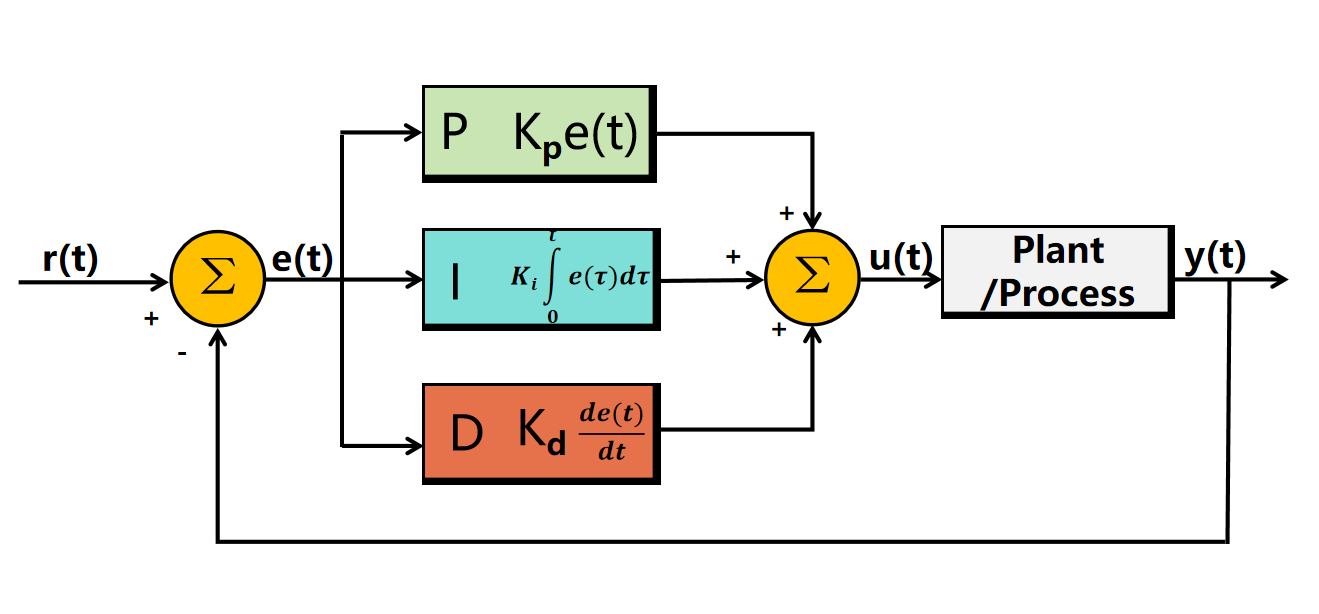
\includegraphics[width=1\textwidth]{p17} % 假设图片文件名为car.pdf或car.png等,位于当前工作目录
	\caption{PID 控制} % 图片标题
	\label{fig:p17} % 用于引用的标签
\end{figure}






\section{基于雷达和相机获取小车坐标数据}
完成了小车的基本控制后,紧接着就是需要通过融合相机和雷达传感器,在CARLA仿真平台上对多目标进行跟踪,获得车辆多个路口的准确轨迹,然后通过再识别技术组合整个轨迹,对车辆进行准确定位,完成车辆的数字孪生系统。下面是步骤。

\subsection{激光雷达检测}

这次设计使用 CARLA 的雷达和相机进行数据融合进行车辆跟踪,获得相对自己车的车辆轨迹,因此需要对 CARLA 的雷达数据集进行 pointPillars 网络训练。本次设计在收集轨迹跟踪数据时,在 Town10 场景中执行 collect lidar dataset.py脚本采集点云训练集,训练集的数据含有点云和3D标签框,都在./multi obj track 目录下便于后期维护管理。脚本首先分别建立存放雷达数据、标签数据文件夹,筛除自行车等非追踪车辆的蓝图,将车分“car ”和“truck”。再获取雷达检测区域内车的信息,并变换到雷达坐标系下,保存为matlab 格式的标签文件,将雷达点云数据转换为 NumPy 数组,并保存为 MATLAB 可以读取的格式,后配置并启动激光雷达传感器,绑定回调 函数用于保存数据,最后销毁传感器和车辆。

\subsubsection{点云数据预处理}
在MATLAB中运行 ‘convertTrainPointCloudToPcd.m‘脚本,首先 获取并确保相关文件夹的路径正确,然后获取数据文件夹下的.mat文件列表, 再逐一读取这些文件,提取点云数据形成pointCloud对象,然后再根据激光 雷达参数重新组该点云数据,最后将重新组织后的点云数据以ASCII格式的 PC文件保存,将点云训练集转化为PCD格式文件;与此同时运行‘convertTrainLabelToTableMat.m‘脚本,先是初始化空表格,再获取、确保相关文件夹的路径正确,然后获取数据文件夹下的.mat文件列表,再一读取这些文件,从中提取汽车和卡车的标签数据并转化为表格行加入到主表格中,最后将主表格保存为CarlaSetLidarGroundTruth.mat 文件,将所有帧的训练标签合并成一个MAT文件。最后会得到如图\ref{fig:p10}展示的数据文件。




\begin{figure}[htbp] % 可以是h(here),t(top),b(bottom),p(page of floats)
	\centering
	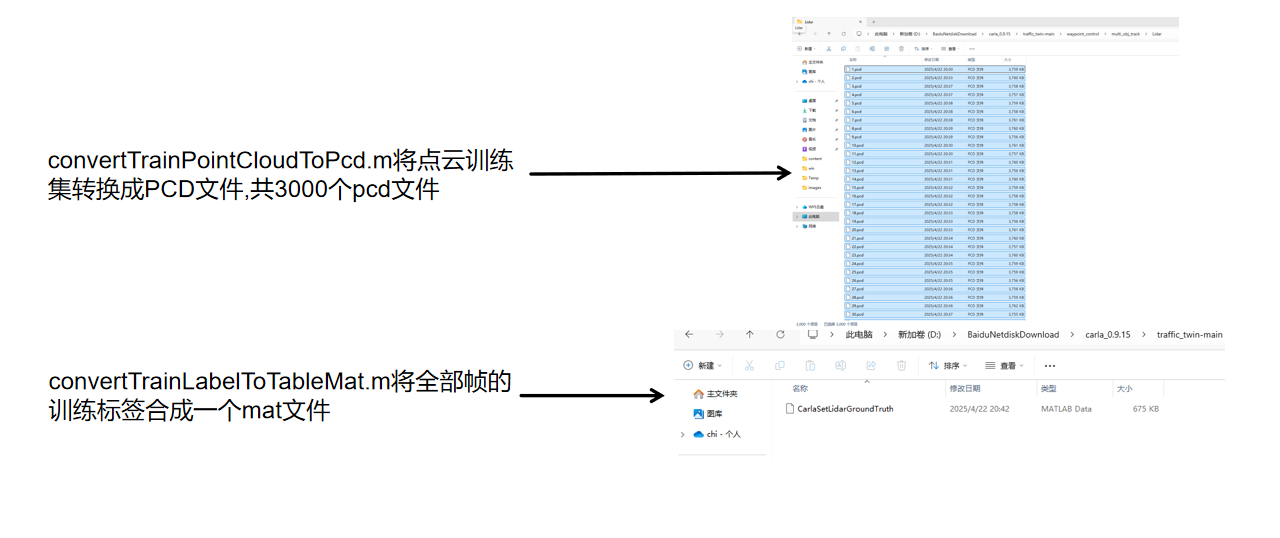
\includegraphics[width=1\textwidth]{p10} % 假设图片文件名为car.pdf或car.png等,位于当前工作目录
	\caption{点云数据预处理} % 图片标题
	\label{fig:p10} % 用于引用的标签
\end{figure}




\subsubsection{训练}
在matlab中运行pointPillarsTrain.m脚本,开始训练如图\ref{fig:p30}!先设置数据路径,加载雷达点云数据和边界框标签,并展示全视图点云;接着定义裁剪参数,裁剪点云并处  理标签;然后拆分数据集为训练集和测试集,保存训练数据为 PCD 文件,创建文件数据存储和框标签数据存储并合并用于训练;之后通过过采样和变换对点云数据增强,增加数据集多样性;再计算锚框,创建 PointPillars 模型;设置训练参数,训练模型并保存检查点;从测试集取点云进行目标检测,可视化检测结果;最后保存训练好的检测模型。将训练好的模型如图\ref{fig:p11}保存在当前目录 (./multi obj track) 下。



\begin{figure}[htbp] % 可以是h(here),t(top),b(bottom),p(page of floats)
	\centering
	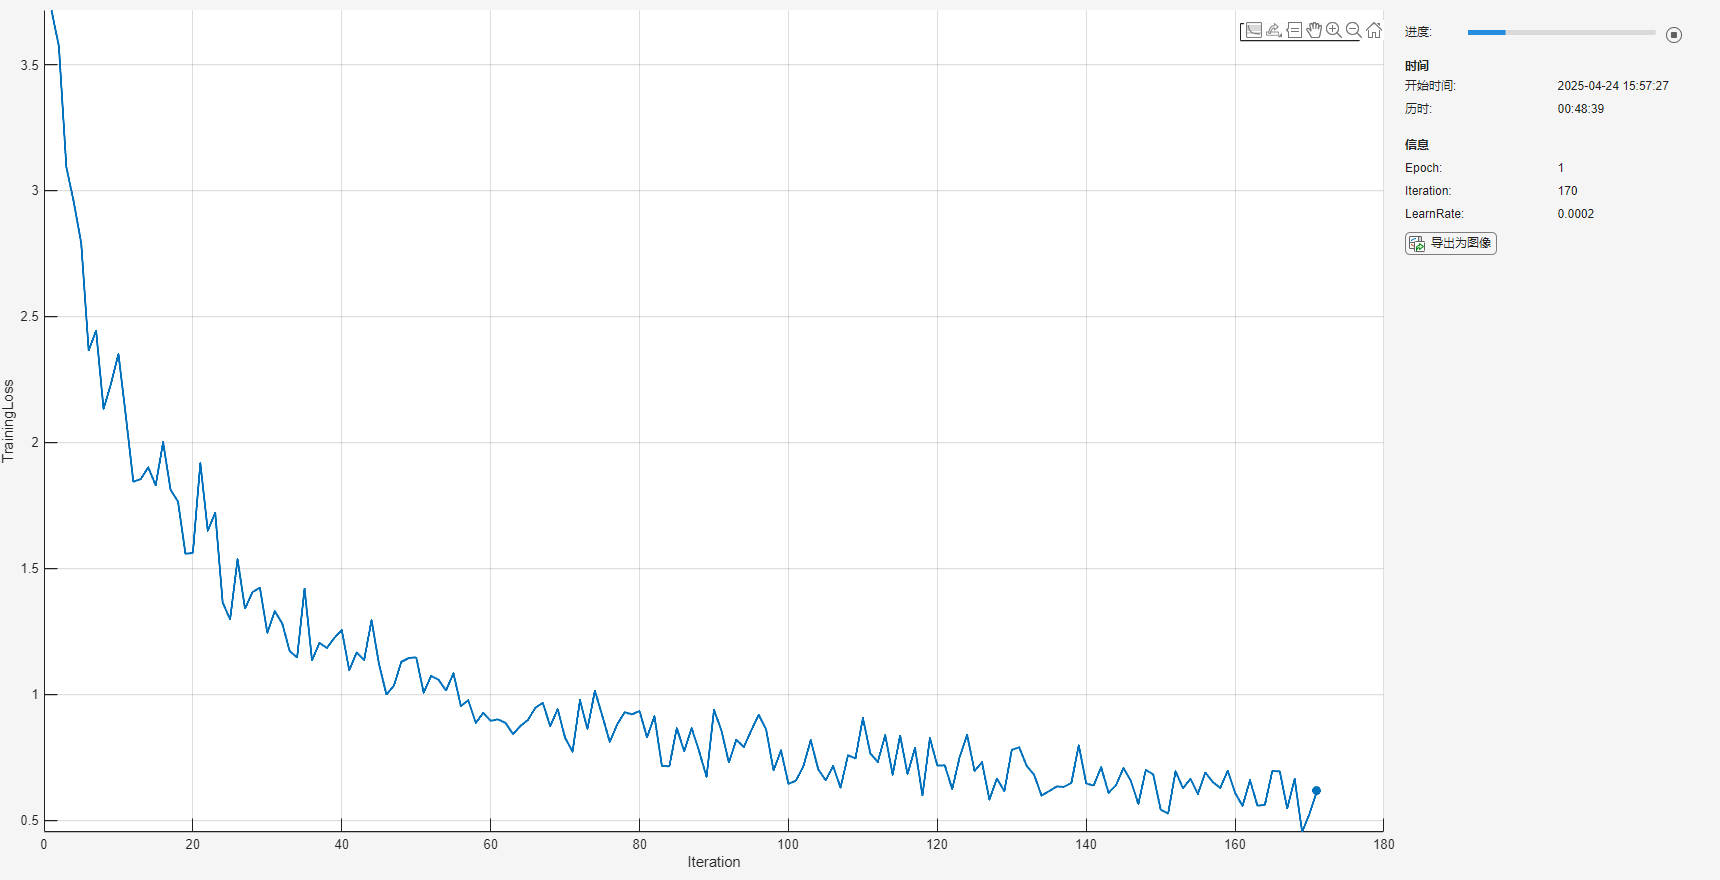
\includegraphics[width=1\textwidth]{p30} % 假设图片文件名为car.pdf或car.png等,位于当前工作目录
	\caption{模型训练中} % 图片标题
	\label{fig:p30} % 用于引用的标签
\end{figure}








\begin{figure}[htbp] % 可以是h(here),t(top),b(bottom),p(page of floats)
	\centering
	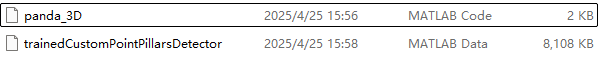
\includegraphics[width=1\textwidth]{p11} % 假设图片文件名为car.pdf或car.png等,位于当前工作目录
	\caption{训练好的模型} % 图片标题
	\label{fig:p11} % 用于引用的标签
\end{figure}






\subsection{激光雷达和摄像头数据的对象级融合}
\subsubsection{收集轨迹跟踪的数据}
Town10 场景,执行collect intersection camera lidar.py收集多目标跟踪的测试数据,其中每个十字路口中心有 1 个激光雷达,雷达周围布局有 6 个 RGB 相机,收集每一帧的 6 个视角的场景图像和点云数据,存放在./multi obj track 中,在 collect intersection camera lidar.py 脚本中,设置DATA MUN = 500,表示收集 500 帧的 6 个视角的场景图像和点云数据如图\ref{fig:p12},方便后续操作。



\begin{figure}[htbp] % 可以是h(here),t(top),b(bottom),p(page of floats)
	\centering
	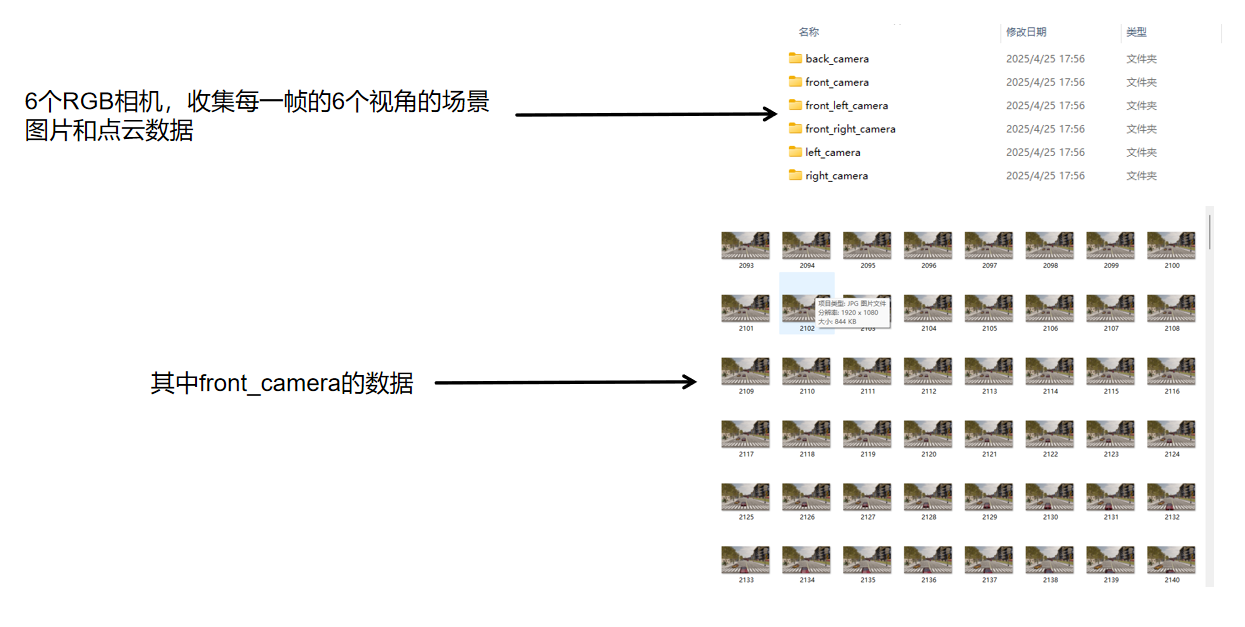
\includegraphics[width=1\textwidth]{p12} % 假设图片文件名为car.pdf或car.png等,位于当前工作目录
	\caption{雷达相机数据} % 图片标题
	\label{fig:p12} % 用于引用的标签
\end{figure}



\subsubsection{数据预处理}


detect3DBoundingBox.m 这个程序是为了在点云数据中搜索汽车并为它们附加 3D 标签而生的。它首先会从特定的位置导入预训练的PointPillars检测模型。然后,该程序会找到某一个文件夹下的所有 .mat 文件。对于每一个这样的文件,它会先寻找有效点云。如果存在有效的点云,则会提取出这些点云,并组织成点云对象。然后用探测器来识别物体,生成边框、得分以及标签,最后以可视化的方式呈现,并保存回原文件。

detect2DBoundingBox.m这个脚本的作用是在图像中识别车辆为其贴上2D加载数据和加载图像。使用YOLOv4探测器识别对象,但排除“交通灯”标签的目标检测。最后将有效的检测结果保存到原始文件中。



\subsubsection{数据融合,获取轨迹}

multiObjectTracking.m 对跟踪车辆进行可视化。首先设置路径并加载文件,对显示和轨迹对象进行初始化;接着在数据帧处理循环里,从数据载入与时间戳验证开始,依次执行获得检测数据、整合检测结果、对目标进行跟踪、展示结果、以及轨迹更新与存储; 最终将完整的轨迹数据存储到特定文件夹供后续评估与分析用,生成 trackedData.mat。

\subsubsection{坐标转换}

获得的轨迹是以自车的坐标,但是本次设计假设自车是静止在十字路口中心(实际 并不存在),而雷达和摄像机都是安装在自车上的,即对自车都有一个相对的位置,在该 示例中雷达对于汽车的相对位置是[0, 0, 0],但是在本课题中雷达高出一定的高度。convertTrackToCarla-Coordinate.m将坐标转化成了CARLA场景中的轨迹,用的是相对 的自车坐标的,所以(x,y)是对的。


通过以上的(1)(4)步,可以收集到 500 帧的轨迹跟踪视频,如图\ref{fig:p13}所示(在 collect intersection camera lidar.py 中设定的参数 DATA MUN = 500)。




\begin{figure}[htbp] % 可以是h(here),t(top),b(bottom),p(page of floats)
	\centering
	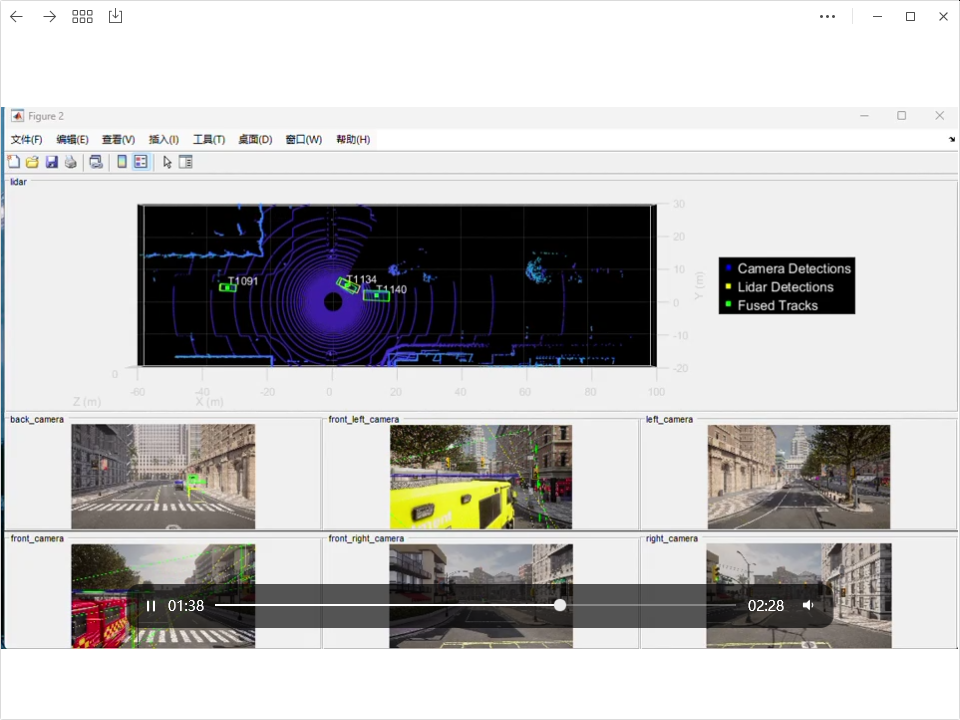
\includegraphics[width=1\textwidth]{p13} % 假设图片文件名为car.pdf或car.png等,位于当前工作目录
	\caption{收集轨迹跟踪视频其中一帧} % 图片标题
	\label{fig:p13} % 用于引用的标签
\end{figure}







\subsection{Re-ID网络再识别}
\subsubsection{收集车辆再识别数据集}

首先利用collect reid dataset.py在同样的地点生成车,然后在车的起始端和终 点端各放一个RGB相机与一个语义分割相机,抓取每帧的车辆前后端的方向图以及2D标签。

\subsubsection{数据裁剪}

运行 cropReIDDataSet.m 可以将前后的视角的车辆图像按照2D标签来进行裁剪,同时还将同类车前后的图像放在一起,并最终调整为 224 ×224 的尺寸如图\ref{fig:p14}。



\begin{figure}[htbp] % 可以是h(here),t(top),b(bottom),p(page of floats)
	\centering
	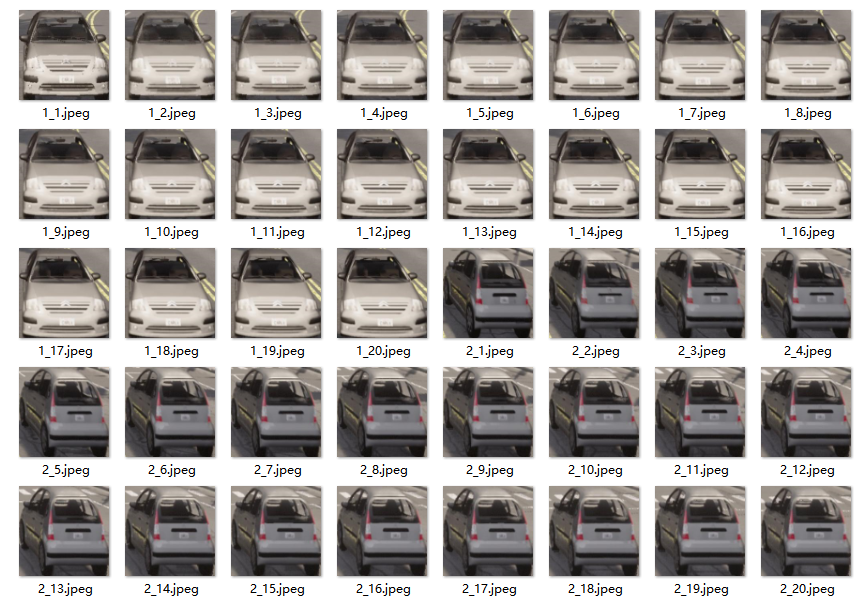
\includegraphics[width=1\textwidth]{p14} % 假设图片文件名为car.pdf或car.png等,位于当前工作目录
	\caption{裁剪后的数据} % 图片标题
	\label{fig:p14} % 用于引用的标签
\end{figure}




\subsubsection{训练}
reIDNetworkTrain.m 采用 imagePretrainedNetwork 函数且选择 resnet50 网络进行训练,此神经网络已经在海量图片上学习到很多的特征描述。
\subsubsection{测试}

把路口1位置监控到的汽车汽车图像以及在路口2位置这个角度的摄像机的照片放一起做再识别reIdentification.m, 换言之第一张照片是需要重新识别的目标,在下一个路口被辨识,从而结合两者的踪迹,最后就可以得到如下\ref{fig:p15}再识别后结果的数据。






\begin{figure}[htbp] % 可以是h(here),t(top),b(bottom),p(page of floats)
	\centering
	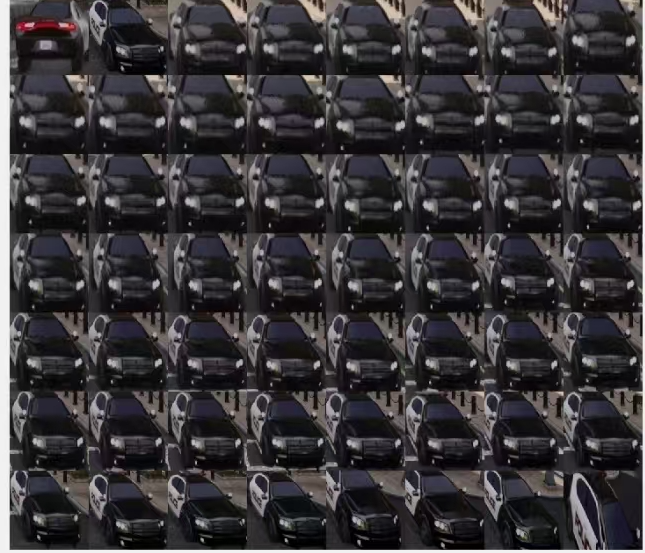
\includegraphics[width=1\textwidth]{p15} % 假设图片文件名为car.pdf或car.png等,位于当前工作目录
	\caption{再识别后数据} % 图片标题
	\label{fig:p15} % 用于引用的标签
\end{figure}









\subsection{路口间车辆轨迹匹配}
\subsubsection{生成可作匹配的轨迹}

多目标跟踪multiObjectTracking.m可视化跟踪的车辆,输出trackedData.mat的同时,也对每一个轨迹对应的车辆进行了图片存储。该图片是通过结合融合的3D框及Yolo检测到的2D框判断为同一辆车后,选取其2D框进行截取,重新形成大小为可进行特征提取的224\times224的图片。

loadAllTraj.m 用于生成特定路口轨迹以及对应车辆的外貌特征。

\subsubsection{车辆轨迹匹配}
现在只是单纯地算出两路口之间所有轨迹车辆的余弦相似度进行匹配,如果路口1有M辆车,路口2有N辆车,生成 M×N 矩阵,大于一定的阈值就认为这两辆车是一辆车。
\subsubsection{运行}
运行 DEMO.m,首先读取配置文件,设置好路径,然后读取各个路口的轨迹文件到cell数组中,再利用匹配算法把不同路口的轨迹根据阈值连接成完整的路线,最后保存匹配完成后的轨迹从而把两个路口的轨迹联系在一起!
\subsection{重复上述步骤}


由于本课题中规定的是多路口目标跟踪检测,而上述步骤仅仅只有 road intersec- tion 1 路口的数据。同时 Town10 场景有 6 个路口,因此需要返回激光雷达摄像头数 据对象级融合的第一步采集轨迹跟踪数据重新运行 collect intersection cameralidar.py,并在该脚本中将 road intersection1改为road intersection 2(后期可改为3或者4或5)进行其余路口的收集数据。最终收集全部数据如图\ref{fig:p18}所示。




\begin{figure}[htbp] % 可以是h(here),t(top),b(bottom),p(page of floats)
	\centering
	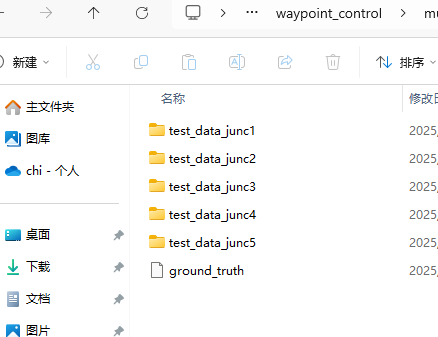
\includegraphics[width=1\textwidth]{p18} % 假设图片文件名为car.pdf或car.png等,位于当前工作目录
	\caption{五个路口数据} % 图片标题
	\label{fig:p18} % 用于引用的标签
\end{figure}






\section{小车轨迹复现}

在上面所说的过程就是对road intersection 1、road intersection 2、road intersection 3 、road intersection 4 和 road intersection 5 这五个十字路口的车辆坐标的收集过程。


\subsection{对轨迹数据的优化}
因该项目中的雷达摄像头位于路口与路口之间,其中既可能不存在小车路口转弯或是直走的轨迹,也可能看不到小车路口转弯或是直走的轨迹。因此,该项目中 evaluator.py 程序用于采用动态时间规整 (DTW) 计算两个路口摄像头中小车轨迹重合程度。
\subsubsection{计算两条轨迹的重合度}
先抽取轨迹的x,y坐标,保证两个轨迹的长度相等(取较小值),利用DTW求出两个轨  迹的距离,算出最大的可能的距离(两个轨迹完全不存在重合)。然后算出它们的相似程2 度并重限制在[0,1]范围内。用动态时间规整(DTW)计算两个轨迹的相似程度。

param truth trajectory: 真实轨迹,格式为 [[x1, y1, t1], [x2, y2, t2], ...]。

param track trajectory: 控制轨迹,格式为 [[x1, y1, z1], [x2, y2, z2], ...]。

param threshold: 判断重合点的位置误差阈值(默认 0.5 米)。

return: 轨迹重合度(0 到 1 之间的值,1 表示完全重合)。

\subsubsection{计算轨迹的多个指标}
其次是计算轨迹的各类指标,本项目做法是首先遍历truth和track键与值,初始化当前车 辆的指标,然后计算当前车辆的误差-计算欧式距离(只考虑x、y),计算当前车辆的轨迹重合度(采用DTW),计算当前车辆的终点误差,然后累加当前车辆的指标并计算平均指标。

平均轨迹重合度(Mean Trajectory Overlap Ratio, TOR)

平均位置误差(Mean Position Error, MPE)

平均最大位置误差(Mean Maximum Position Error, MeanMaxPE)

平均终点误差(Mean Final Position Error, MFPE)

param truth: 车辆的轨迹字典,键为车辆编号,值为 [[x1, y1, t1], [x2, y2, t2], ...]。

param track: 控制车辆所走的轨迹字典,键为车辆编号,值为 [[x1, y1, z1], [x2, y2,z2], ...]。

param threshold: 判断重合点的位置误差阈值(默认 0.5 米)。

return:平均轨迹重合度、平均位置误差、平均最大位置误差和平均终点误差的元组(mean tor,mean error, mean max error, mean fpe)。


\subsubsection{计算所有车辆的误差}
最后对每一辆车的横向误差、纵向误差和延迟列表(如果车辆没有数据,跳过),确保横向误差、纵向误差和延迟的帧数一致,加当前车辆的横向误差、纵向误差和延迟,算平均横向误差、平均纵向误差和平均延迟(如果没有数据,返回 (0.0, 0.0, 0.0))。

计算所有车辆的平均横向误差(Mean Lateral Error, MLE)、平均纵向误差(Mean Longitudinal Error, MLOE)和平均延迟(Mean Delay, MD)。

param lateral errors: 横向误差列表,每个子列表表示一辆车的每一帧的横向误差。

param longitudinal errors: 纵向误差列表,每个子列表表示一辆车的每一帧的纵向误差。

param delays: 延迟列表,每个子列表表示一辆车的每一帧的延迟。

return:平均横向误差、平均纵l向误差和平均延迟的元组(mean lateral error,mean longitudinal error, mean delay)。


\subsection{坐标数据再处理}
\subsubsection{多路口车辆轨迹数据}



在 DEMO.m脚本下把五个路口的全部轨迹都放进去,并运行。DEMO.m 脚本首先加载轨迹数据,对于每个路口的数据集路径,调用 loadAllTraj 函数来加载该十字路口的所有轨迹数据,通过循环所有.mat 如图\ref{fig:p19}(test data junc1 traj 、test data junc2  traj 、test data junc3 traj 、test   data junc4 traj 、test data junc5 traj)文件,然后加载每个文件用来识别不同路口中的轨迹是否为同一辆车的,做完这一步后会调用 linkIdentities 函数,将整个路口的所有轨迹进行关联匹配,形成全局唯一的车辆轨迹。最后将匹配好的轨迹数据保存至 traj.mat 文件中。

总体上这一段代码是对多个路口的车辆轨迹进行匹配关联,形成全局唯一的轨迹便于后面对车辆轨迹的还原。


\begin{figure}[htbp] % 可以是h(here),t(top),b(bottom),p(page of floats)
	\centering
	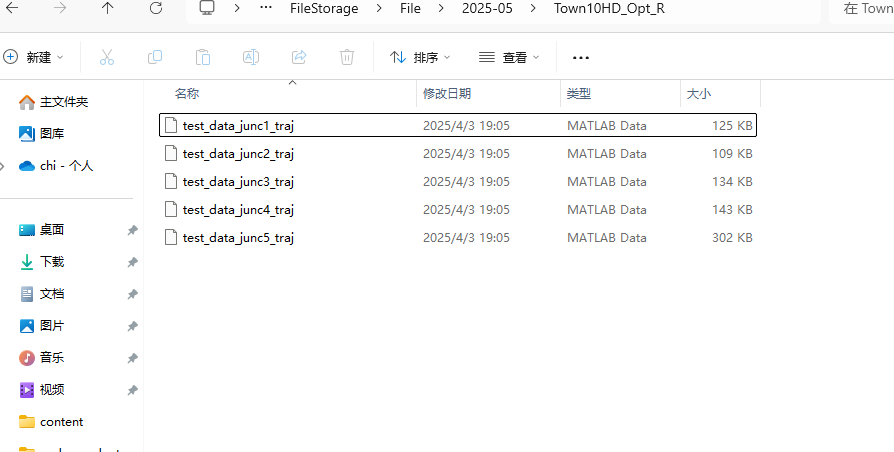
\includegraphics[width=1\textwidth]{p19} % 假设图片文件名为car.pdf或car.png等,位于当前工作目录
	\caption{五个路口数据} % 图片标题
	\label{fig:p19} % 用于引用的标签
\end{figure}






\subsubsection{转化轨迹数据格式}
上述步骤得到的5个路口车辆轨迹坐标数据,还不符合本课题车辆轨迹的复现需要,在Drive.py脚本中,在进行车辆轨迹复现的同时,读取的是名为Waypoints.txt文件夹中的数据。因此,我们需要将上述得到的5个路口车辆轨迹坐标数据转换为int(float或double)类型的坐标数据存储到Waypoints.txt中。

首先,对小车的轨迹进行处理,从traj.mat文件中读取车辆的行驶轨迹信息,一条轨迹有三维坐标点以及时间戳 。检测轨迹起始点,如果距离较远则剔除。对于同一条车辆轨迹在多个路口出现的情况,则通过 Carla 路径规划方法生成过渡路线并用插值法保证时间戳的连续性。采用fastdtw算法计算追踪轨迹与真实轨迹的最佳匹配,评价指标包括平均位置误差,最大定位误差,最后位置误差和轨迹覆盖率。最后,将处理后的汽车轨迹按时间戳升序排列,并保存到 Waypoints.txt文件,如图\ref{fig:p20}所示。


\begin{figure}[htbp] % 可以是h(here),t(top),b(bottom),p(page of floats)
	\centering
	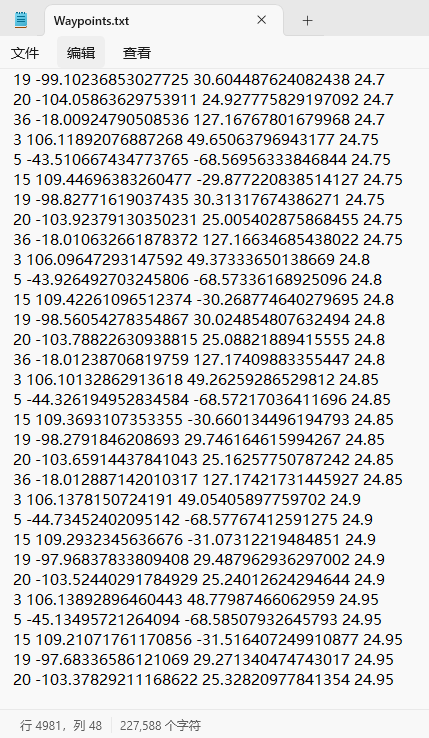
\includegraphics[width=0.5\textwidth]{p20} % 假设图片文件名为car.pdf或car.png等,位于当前工作目录
	\caption{小车坐标轨迹数据} % 图片标题
	\label{fig:p20} % 用于引用的标签
\end{figure}









\subsection{开始复现}

经过以上的准备,项目已具备预测小车在两个路口到另一个路口之间的轨 迹能力,包括小车可能未在路口转弯或未直行的情况。因此,在通过evaluator.py程序优化和预测小车位置数据的前提下,执行Drived.py脚本,调用Waypoints .txt 中的数据重现小车轨迹如图\ref{fig:p21}所示,图片仅是本次的设计重制视频当中的一个镜头,从而使得小车的基线已经达到了项目要求5\%以上的标准。


\begin{figure}[htbp] % 可以是h(here),t(top),b(bottom),p(page of floats)
	\centering
	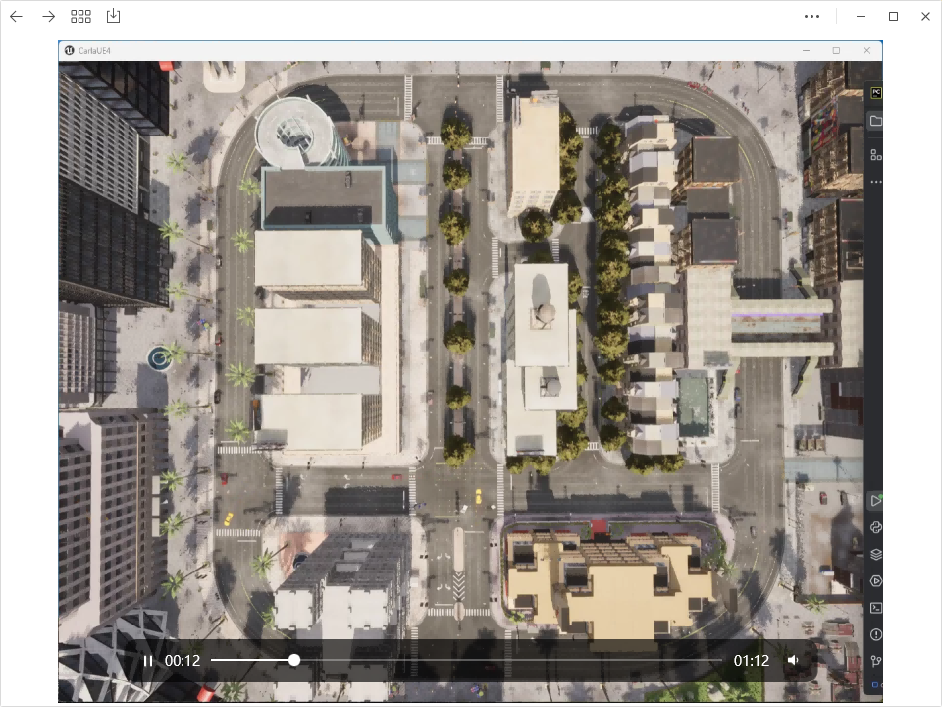
\includegraphics[width=1\textwidth]{p21} % 假设图片文件名为car.pdf或car.png等,位于当前工作目录
	\caption{小车轨迹的复现} % 图片标题
	\label{fig:p21} % 用于引用的标签
\end{figure}






\section{结果分析}

此次毕业设计的工作是关于针对智慧交通背景下的多目标跟踪算法及评估,主要对检测跟踪模型进行改进,使得其在许多性能方面都得到了较为显著的提升。实验结果显示, 改进后的模型在这 MOTA、 MOTP 和 IDS等重要指标上,都高于Baseline有5\%。同时,也通过可视化手段直观展示了改进后的模型效果。以下,本次设计就展现性 能指标、优化目标和模型改进及其结果分析。








\subsection{结果性能分析}
\subsubsection{性能指标}
TT(Trajectory Tracking):轨迹跟踪,是指控制车辆沿着给定轨迹行驶,轨迹定义在时间域上,需要同时控制车辆的横向和纵向运动,以贴合给定轨迹并匹配其时间。

DT(Detection and Tracking):检测与跟踪,这类方法依赖于从传感器数据(如摄像头、激光雷达等)中检测车辆,然后对检测到的车辆进行跟踪,以生成轨迹。

GT(Generation and Tracking):生成与跟踪,这可能涉及使用预测模型或轨迹生成算法来生成车辆的预期轨迹,然后将这些生成的轨迹与实际跟踪数据相结合,以提高轨迹预测的准确性和完整性。

TOR(Trajectory Overlap Rate):轨迹重合度,表示跟踪轨迹与真实轨迹的重合程度,通常用来衡量轨迹跟踪的准确性。

MPE(Mean Position Error):平均位置误差,指跟踪轨迹与真实轨迹之间位置误差的平均值,用于评估轨迹跟踪的精度。

MaxPE(Maximum Position Error):最大位置误差,指跟踪轨迹与真实轨迹之间位置误差的最大值,用于评估轨迹跟踪中最坏情况下的误差。

FPE(Final Position Error):最终位置误差,指跟踪轨迹与真实轨迹在轨迹终点的位置误差,用于评估轨迹跟踪的最终精度。

MLE(Mean Longitudinal Error):平均纵向误差,指沿轨迹方向的纵向误差的平均值,用于评估车辆在纵向上的跟踪精度。

MLOE(Mean Lateral Offset Error):平均横向偏移误差,指垂直于轨迹方向的横向偏移误差的平均值,用于评估车辆在横向上的跟踪精度。

MD(Mean Deviation):平均偏差,指跟踪轨迹与真实轨迹之间的平均偏差,综合反映了轨迹跟踪的整体误差水平。

MOTA(Multi-Object Tracking Accuracy):多目标跟踪精度,综合考虑了跟踪的准确性和完整性。

MOTP(Multi-Object Tracking Precision):多目标跟踪精度,衡量跟踪轨迹与真实轨迹的匹配程度。

Int.(Intersection):意为“交叉路口”或“交汇点”。

IDS:综合考虑了跟踪的准确性和稳定性的指标。

FP(False Positives):误检数量。

FN(False Negatives):漏检数量。

MT(Mostly Tracked):大部分时间被跟踪的目标数量。

ML(Mostly Lost):大部分时间丢失的目标数量。

Fragmentation:轨迹碎片化程度。

Precision:精确率。

Recall:召回率。
\subsubsection{优化目标}


按照课题规定,改进后的模型必须在3项性能指标至少超越Baseline5\%。本次设计通过对检测算法的改进,对数据融合策略的改良以及使用更高级的跟踪算法来实现对现有模型的改进。







\subsection{模型优化}

识别算法优化:基于PointPillars深度学习网络模型对激光雷达进行3D目标识别,同时利用预训练的YOLOV4模型对图像进行2D目标识别,提升了识别精度与效率。


数据融合策略改进:基于激光雷达与摄像头数据进行物体级的融合,采取卡尔曼滤波器对目标轨迹进行平滑处理,降低了轨迹碎片化问题。


跟踪算法优化:增加基于 ReID(Re-Identification)的再识别功能,利用车辆外观特 征余弦相似度进行跨多路口车辆轨迹比对,增强跟踪稳定性和准确性。

\subsubsection{模型优化一:跟踪}

通过插值算法来对轨迹点变得更为平滑连续,从而用来填补轨迹空隙或简化多余的点,让轨迹追踪的准确和流畅程度更高。

通过调用 Carla 的全局路径规划器来求取车辆在各个不同位置间的最短路径,给轨迹跟踪提供一个比较合理的路径规划。

采用DTW算法计算所跟踪到的轨迹与原始轨迹之间的相似性,从而判断轨迹的追踪精度和稳定性。

统计多种轨迹跟踪评价指标包括平均轨迹重合度(TOR)、平均位置误差(MPE)、平均最大位置误差(MeanMaxPE)以及平均终点误差(MFPE),从而综合评价轨迹跟踪的效果。

通过对优化前后的模型进行评测,得到了以下如表~\ref{tab:trajectory_com}和如表~\ref{tab:tracking_comparison}性能指标的统计结果:

\begin{table}[h]
	\centering
	\caption{Trajectory Overlap Rate and Vehicle Control Indicators}
	\label{tab:trajectory_com}
	\resizebox{\textwidth}{!}{%
		\begin{tabular}{|l|c|c|c|c|c|c|c|c|c|c|c|c|c|}
			\hline
			\textbf{Scene} & \textbf{Int.} & \textbf{Rcll} & \textbf{Prcn} & \textbf{FTR} & \textbf{FP} & \textbf{FN} & \textbf{IDS} & \textbf{MT} & \textbf{ML} & \textbf{RMOTA} & \textbf{RMOTP} \\ \hline
			\multicolumn{12}{|c|}{优化后 Town10} \\ \hline
			Town10  & 1 & 30.1025 & 59.9258 & 0.5106 & 216 & 750 & 18 & 0.0000 & 37.5000 & 8.2945 & 79.9222 \\ \hline
			Town10  & 2 & 64.8065 & 61.5385 & 1.1027 & 450 & 391 & 21 & 55.5556 & 33.3333 & 22.4122 & 86.7746 \\ \hline
			Town10  & 3 & 63.2135 & 45.4407 & 1.1887 & 359 & 174 & 15 & 0.0000 & 25.0000 & -15.8562 & 86.9053 \\ \hline
			Town10  & 4 & 65.8206 & 96.7662 & 0.0369 & 13 & 202 & 20 & 40.0000 & 20.0000 & 60.2369 & 89.0919 \\ \hline
			Town10  & 5 & 41.4035 & 90.0763 & 0.0580 & 13 & 167 & 10 & 50.0000 & 0.0000 & 33.3333 & 88.2471 \\ \hline
			\multicolumn{12}{|c|}{优化前 Town10} \\ \hline
			Town10  & 1 & 30.6653 & 59.7166 & 0.7960 & 398 & 1334 & 28 & 8.3333 & 50.0000 & 8.5239 & 84.6488 \\ \hline
			Town10  & 2 & 56.4410 & 70.6095 & 1.1380 & 569 & 1055 & 29 & 13.3333 & 2666467 & 31.7506 & 81.0192 \\ \hline
			Town10  & 3 & 51.9805 & 75.6714 & 0.6160 & 308 & 885 & 17 & 14.2857 & 35.7143 & 34.3464 & 84.2826 \\ \hline
			Town10  & 4 & 52.1930 & 86.1427 & 0.2680 & 134 & 763 & 50 & 27.2727 & 36.3636 & 40.6642 & 88.6035 \\ \hline
			Town10  & 5 & 45.4243 & 62.2719 & 1.6540 & 827 & 1640 & 35 & 12.5000 & 37.5000 & 16.7388 & 86.0825 \\ \hline
		\end{tabular}
	}
\end{table}


\begin{table}[htbp]
	\centering
	\caption{Multi-objective Tracking Evaluation Comparison}
	\label{tab:tracking_comparison}
	\begin{tabular}{@{}llcccccc@{}}
		\toprule
		\textbf{Scene} & \textbf{Metric} & \textbf{Optimized Town10} & \textbf{Before Optimization Town10} \\
		\midrule
		\multirow{8}{*}{Town10} 
		& Rcll & 64.8065 (Int. 2) & 86.1427 (Int. 4) \\
		& Pren & 61.5385 (Int. 2) & 86.1427 (Int. 4) \\
		& FTR & Better in Int. 1 and 2 & Generally lower, 52.4243 (Int. 5) \\
		& FP & Lower in Int. 3 and 5 & Higher in Int. 1 and 2 \\
		& FN & Higher in Int. 3 and 4 & Higher in Int. 1 and 3 \\
		& IDS & Fewer & 35 (Int. 5) \\
		& MT & Better in Int. 2 and 3 & 40.0000 (Int. 4) \\
		& RMOTA/RMOTP & 79.9222 (RMOTP, Int. 2) & 84.2826 (RMOTP, Int. 4) \\
		\bottomrule
	\end{tabular}
\end{table}



结合比较:
若注重追踪准确率(Rcll)及精度(Pren),优化前Town10高密度度和复杂地形场景(如第三个和第四个交叉口)下表现得更优秀。重视特征轨迹召回率 (FTR)和假阳性率(FP),优化后Town10在平坦的道路和稀疏建筑场景(如同一个和第 二个交叉口)下表现更加优异。身份切换(IDS)和绝大部分轨迹(MT)指标,优化后Town10 在目标身份维持以及连续跟踪方面具有相对的优势。在RMOTA和RMOTP综合评价指 标方面,优化后Town10和优化 前Town10在不同交叉口各有所长,但总体来看优化后Town10较为占优势。














\subsubsection{模型优化二:复现}

通过对车辆进行车身特征(例如多视角图像)与语义分割的采集,为轨迹重现提供了更多的车身特征,能够在不同的环境中有效地识别并重现车辆的轨迹。

对多个交叉口的轨迹数据进行加载、处理,应用匹配算法将不同路口间的轨迹进行拼接,形成全域唯一车辆轨迹,提高了还原轨迹的连贯性与整体性。

给出了衡量轨迹回放精度的指标及办法,例如根据轨迹重叠率、距离误差等指标的计算可对轨迹回放精确程度进行客观评价并指导对轨迹回放算法的改进。


通过对优化前后的模型进行评测,得到了以下表~\ref{tab:trajectory_comparisons}和表~\ref{tab:trajectory_comparison}性能指标的统计结果:


\begin{table}[h]
	\centering
	\caption{Trajectory Overlap Rate and Vehicle Control Indicators}
	\label{tab:trajectory_comparisons}
	\resizebox{\textwidth}{!}{%
		\begin{tabular}{|c|c|c|c|c|c|}
			\hline
			\textbf{Scene} & \textbf{Type} & \textbf{TOR(\%)} & \textbf{MPE(m)} & \textbf{MaxPE(m)} & \textbf{FPE(m)} \\ \hline
			优化前 Town10 & TT-DT & 50.2143 & 79.5798 & 33.1382 & 19.8970 \\ \hline
			& TT-GT & 18.4326 & 59.3773 & 79.6541 & 64.0980 \\ \hline
			& Control & MLE: 2.1889, MLOE: 0.5345, MD: 1.2015 \\ \hline
			优化后 Town10 & TT-DT & 10.8957 & 82.4108 & 105.8893 & 105.0854 \\ \hline
			& TT-GT & 34.4533 & 52.5575 & 36.0566 & 31.4600 \\ \hline
			& Control & MLE: 1.9835, MLOE: 0.2614, MD: 1.3780 \\ \hline
		\end{tabular}
	}
\end{table}


\begin{table}[htbp]
	\centering
	\caption{Trajectory Tracking Performance Comparison}
	\label{tab:trajectory_comparison}
	\begin{tabular}{@{}lcccccc@{}}
		\toprule
		\textbf{Scene} & \textbf{Type} & \textbf{TOR(\%)} & \textbf{MPE(m)} & \textbf{MaxPE(m)} & \textbf{FPE(m)} \\
		\midrule
		\multicolumn{2}{l}{\textbf{Optimized Town10}} \\
		\quad TT-DT & & 10.8957 & 82.4108 & 105.8893 & 105.0854 \\
		\quad TT-GT & & 34.4533 & 52.5575 & 36.0566 & 31.4600 \\
		\midrule
		\multicolumn{2}{l}{\textbf{Before Optimization Town10}} \\
		\quad TT-DT & & 50.2143 & 79.5798 & 33.1382 & 19.8970 \\
		\quad TT-GT & & 18.4326 & 59.3773 & 79.6541 & 64.0980 \\
		\midrule
		\multicolumn{2}{l}{\textbf{Control Indicators}} \\
		& Optimized & \multicolumn{4}{l}{MLE: 1.9835, MLOE: 0.2614, MD: 1.3780} \\
		& Before Optimization & \multicolumn{4}{l}{MLE: 2.1889, MLOE: 0.5345, MD: 1.2015} \\
		\bottomrule
	\end{tabular}
\end{table}

总体评价:
在Town10的TT-DT场景中优化前后轨迹重合率(TOR)与终点误差(FPE)上较为优秀,但是在平均位置误差(MPE)上略微低于优化后Town10的TT-DT场景,优化后Town10的TT-GT场景在平均位置误差(MPE)、最大位置误差(MaxPE)以及最终位置误差(FPE)都优于该优化后Town10的TT-DT场景,说明对于优化后Town10来说,TT-GT的方法进行轨迹预测效果较好。

结果:
在注重轨迹重合度(TOR)与最终位置误差(FPE)的同时,优化之前的Town10的TT-DT场景效果更佳。在注重平均位置误差(MPE),最大位置误差(MaxPE)及最终位置误差(FPE)的时候,优化后的Town10的TT-GT场景的效果更好 。


















